\documentclass{article}

\usepackage{amsmath,amssymb,graphicx,geometry,enumitem,caption,subcaption}
\usepackage{xepersian}

\newcounter{qnumber}
\setcounter{qnumber}{1}

\newcommand{\Q}{
\textbf{سوال \theqnumber)}
\stepcounter{qnumber}
}

\setlength{\parindent}{0mm}
\setlength{\parskip}{3mm}
\settextfont{XB Niloofar}

\begin{document}

\begin{center}
\large

به نام او

آزمون پایان ترم سیگنال ها و سیستم ها
\end{center}

\hrulefill

\large


سیگنال 
$
x[n]
$
به ورودی بلوک دیاگرام زیر داده می‌شود:
\begin{center}
\includegraphics[width=90mm]{block.pdf}
\end{center}
که در آن، 
$
H(e^{j\omega})
$
در یک دوره تناوب به صورت زیر است:

\begin{center}
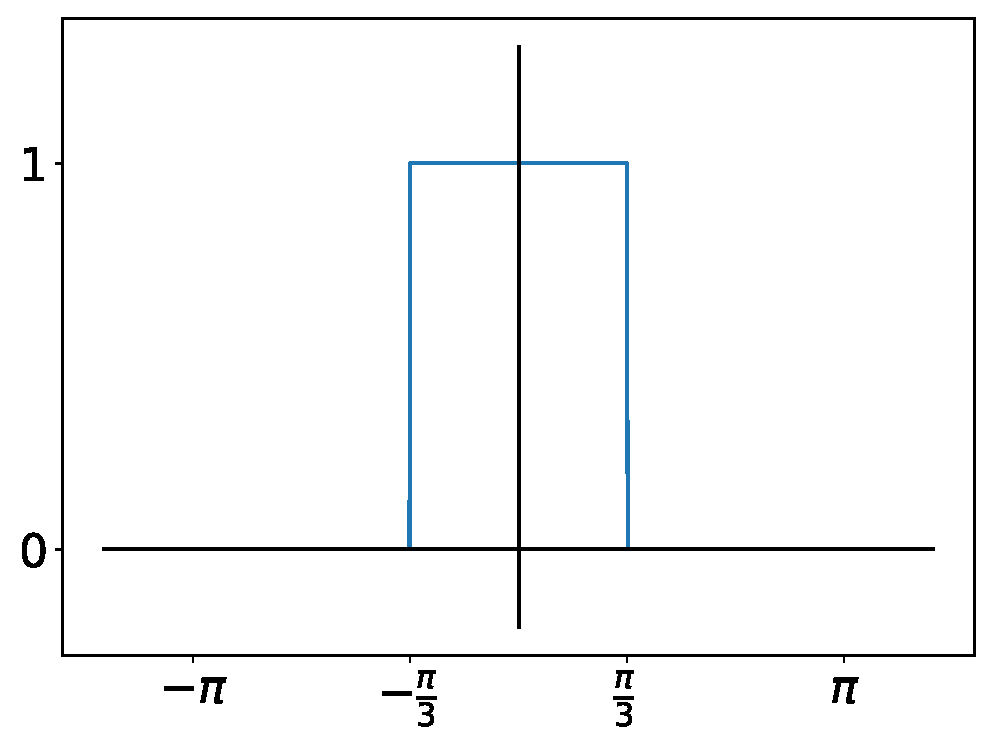
\includegraphics[width=70mm]{final_h}
\end{center}

رابطه‌ی تبدیل فوریه‌های ورودی و خروجی این سیستم را بیابید.

\end{document}